\section{Sprint 7: Pulido y cierre}
\label{sec:pulido-cierre}

Esta último sprint se dedicó a pulir el sistema en todos sus puntos débiles, que eran: mejorar la calidad visual de los sitios generados, consolidar la infraestructura de producción y completar los workflows de n8n que quedaban pendientes. Por infraestructura de producción se entienden los cambios que hacen que el proyecto sea útil fuera del entorno de desarrollo, como por ejemplo la migración a una base de datos más robusta como PostgreSQL para soportar accesos concurrentes de múltiples usuarios, la gestión automática de contenedores Docker activos o la monitorización diaria del sistema. Es decir, no se añadieron funcionalidades realmente nuevas, sino que se llevaron las existentes a un nivel de madurez adecuado para la entrega.


\subsection{Sistema de presets visuales}
\label{subsec:sistema-presets-visuales}

Uno de los principales problemas durante todo el desarrollo fue que los proyectos tendían a parecerse entre si visualmente, independiente del tipo de contenido de la API, del prompt del usuario y del sitio generado. Para resolverlo se creó el módulo \textbf{utils/llm/design}, organizado en tres ficheros con responsabilidades distintas. Estos ficheros eran presets.py, snippets.py y theme\_rules.py.

El fichero \texttt{presets.py} define un catálogo de estilos visuales completos y muy distintos entre sí. Cada preset describe la paleta de colores, el tipo de layout, la estética de los componentes y las palabras clave del prompt del usuario que deben activarlo. Los presets disponibles en este sprint se muestran en la Tabla~\ref{tab:presets-visuales}:

\begin{table}[H]
    \centering
    \begin{tabular}{|l|l|p{5cm}|}
        \hline
        \textbf{Preset} & \textbf{Estética} & \textbf{Palabras clave activadoras} \\
        \hline
        Neo Terminal & Cyberpunk, fondo negro, acento neón & Terminal, dark, gaming, futurista \\
        \hline
        Bento Pop & Rejilla asimétrica, colores vivos & Mosaico, asimétrico \\
        \hline
        Quiet Editorial & Tipografía protagonista, estética revista & Por defecto para blogs \\
        \hline
        Magazine Split & Gran imagen dividida, tipografía impactante & Por defecto para catálogos \\
        \hline
        Glass Orbit & Glassmorphism, fondos oscuros, traslúcidos & Por defecto para portfolios \\
        \hline
    \end{tabular}
    \caption{Presets visuales disponibles en el módulo de diseño}
    \label{tab:presets-visuales}
\end{table}

Cada tipo de sitio tiene asignado un preset por defecto que se aplica cuando el prompt del usuario no contiene ningún estilo descrito, garantizando que el resultado siempre tenga una identidad visual coherente con el tipo de contenido.

El fichero \texttt{snippets.py} complementa los presets con fragmentos de HTML concretos y válidos para cada estilo: cards, heros y filas de listado con las clases Tailwind exactas que corresponden a cada preset. Estos snippets se incluyen en los prompts de generación de templates como ejemplos de referencia visual, asegurando que el LLM produzca código coherente con el estilo elegido.

El fichero \texttt{theme\_rules.py} contiene clases base para contenedores, cards, botones, badges y tipografía, junto con reglas críticas de uso de color para evitar que el LLM genere clases Tailwind inválidas, como \texttt{bg-\#111111} en lugar de la sintaxis correcta \texttt{bg-[\#111111]}.

\subsection{Migración a PostgreSQL}
\label{subsec:migracion-postgresql}

Durante todo el desarrollo, WebBuilder había utilizado SQLite como base de datos, lo cual era suficiente para el entorno de desarrollo pero inadecuado para producción. En este sprint se realizó la migración a PostgreSQL, que ofrece mayor robustez, soporte para accesos concurrentes y mejor rendimiento con volúmenes de datos crecientes.

La configuración en \texttt{settings.py} se actualizó para leer los parámetros de conexión desde variables de entorno: nombre de la base de datos (\texttt{DB\_NAME}), usuario (\texttt{DB\_USER}), contraseña (\texttt{DB\_PASSWORD}), host (\texttt{DB\_HOST}) y puerto (\texttt{DB\_PORT}, por defecto \texttt{5432}). La configuración anterior de SQLite se migró a la nueva base de datos. Las migraciones existentes se aplicaron sobre la nueva base de datos, conservando los logs y métricas generados durante el desarrollo. Tras la migración, el esquema completo de la base de datos quedó de la siguiente manera:

\begin{figure}[H]
    \centering
    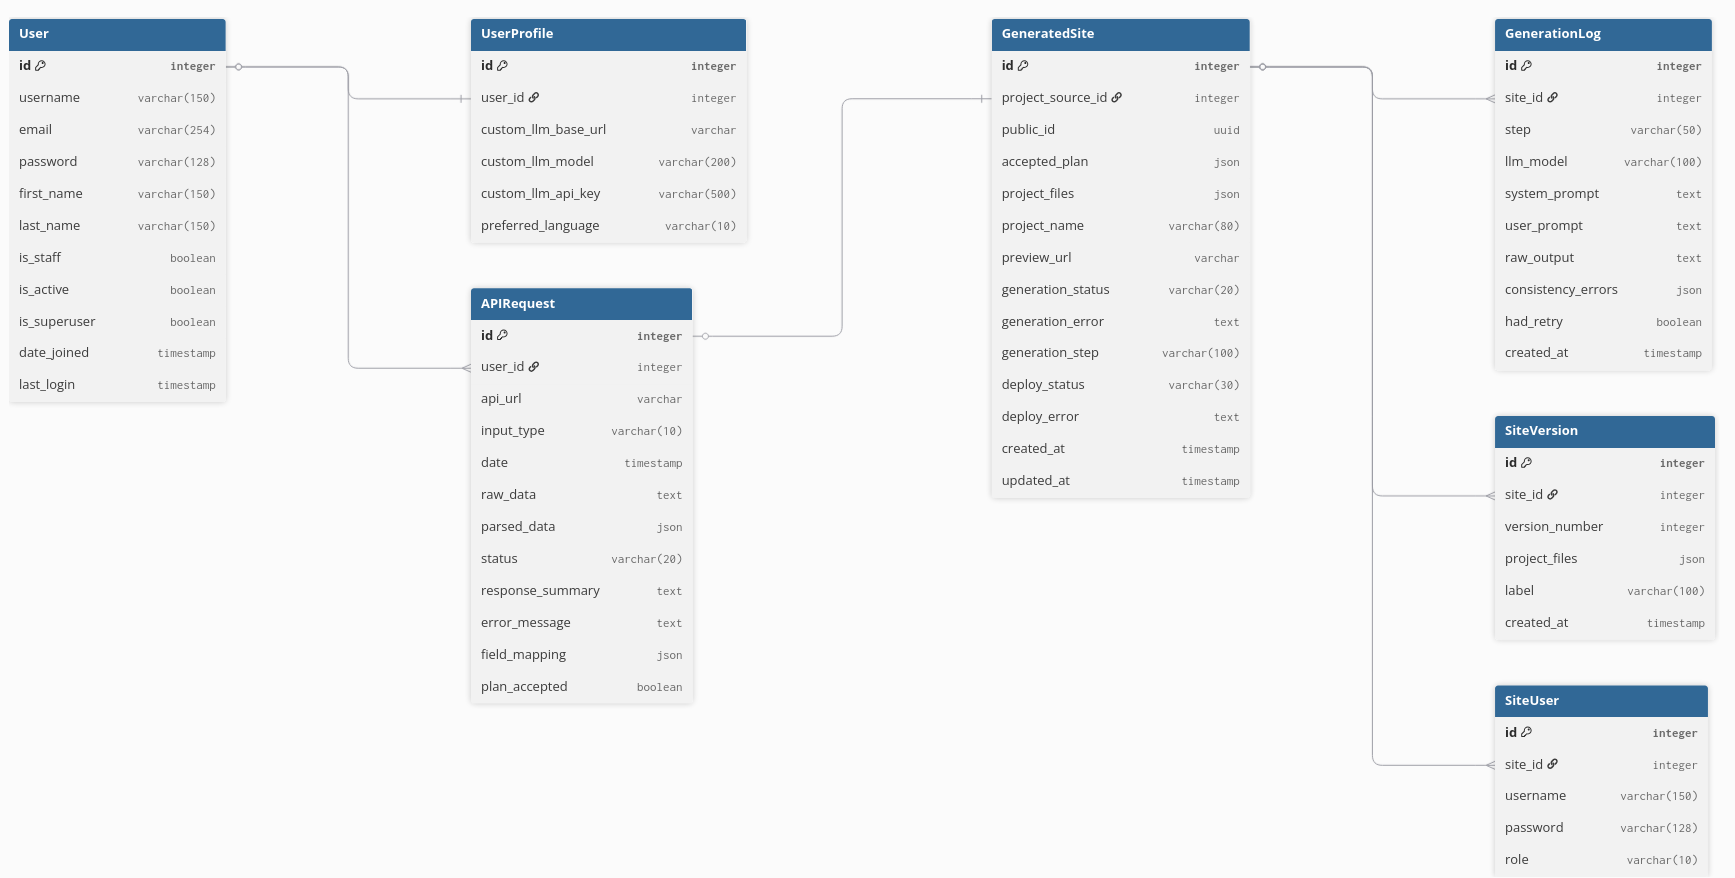
\includegraphics[width=\textwidth]{img/diagramaER.png}
    \caption{Esquema final de la base de datos}
    \label{fig:Esquema final de la base de datos}
\end{figure}


\subsection{Workflow generation-done}
\label{subsec:workflow-generation-done}

Con la base de notificaciones ya preparada desde el fichero \\ \texttt{utils/generator/notifications.py}, se implementó el workflow de n8n \emph{generation-done}. Este workflow se activa mediante un webhook al que Django llama en cuanto termina la generación de un sitio, enviando un payload con los datos relevantes: email y nombre del usuario, título y tipo del sitio generado, URL de la API original, URL del preview si ya está desplegado, URL de descarga del ZIP, número de campos e items procesados, duración de la generación en segundos y modelo de LLM utilizado.
n8n recibe este payload y envía automáticamente un correo de notificación al usuario informándole de que su sitio está listo. La llamada al webhook se realizó de forma completamente transparente al flujo principal: si n8n no estaba disponible o la llamada fallaba, la excepción se capturaba silenciosamente mediante un bloque \texttt{try/except} y la generación continuaba con normalidad.

\begin{figure}[H]
    \centering
    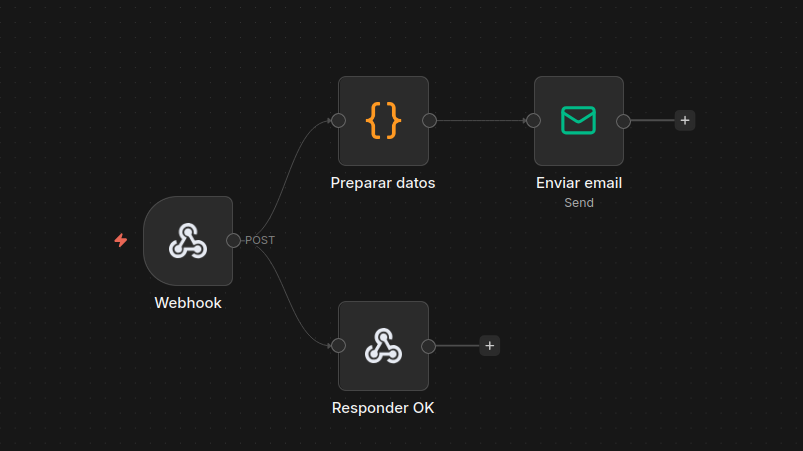
\includegraphics[width=0.7\textwidth]{img/n8n/generation-done.png}
    \caption{Workflow generation done}
    \label{fig:Workflow generation done}
\end{figure}

\subsection{Workflow health-check}
\label{subsec:workflow-health-check}

El workflow de \emph{health-check} se configuró para ejecutarse automáticamente cada día mediante un nodo \emph{Schedule Trigger} de n8n. Su función es verificar que el sistema sigue operativo realizando una petición HTTP a la URL principal de WebBuilder y comprobando que la respuesta es correcta. Si la verificación falla, n8n envía una alerta por correo al administrador del sistema con información sobre el error detectado. Aunque su uso fue puntual durante las últimas fases 
de desarrollo, ayudó a la monitorización del sistema para comprobar su correcto funcionamiento.

\begin{figure}[H]
    \centering
    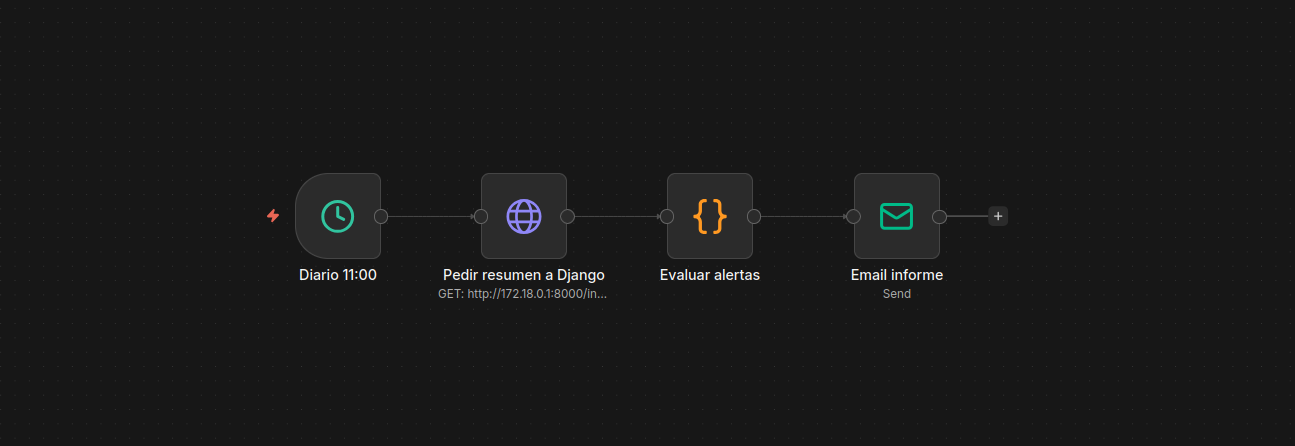
\includegraphics[width=\textwidth]{img/n8n/health-check.png}
    \caption{Workflow health check}
    \label{fig:Workflow health check}
\end{figure}


\subsection{Workflow auto-shutdown}
\label{subsec:workflow-auto-shutdown}

El workflow de \emph{auto-shutdown} resolvió un problema operativo importante: los contenedores Docker de los sitios generados permanecían activos indefinidamente aunque nadie los estuviera usando, consumiendo recursos del servidor. Este workflow se ejecuta de forma programada cada hora, consulta la lista de contenedores activos con el prefijo \texttt{wb\_} y detiene aquellos que están inactivos. Esto permite mantener el servidor limpio y los recursos disponibles para nuevas generaciones sin intervención manual.

\begin{figure}[H]
    \centering
    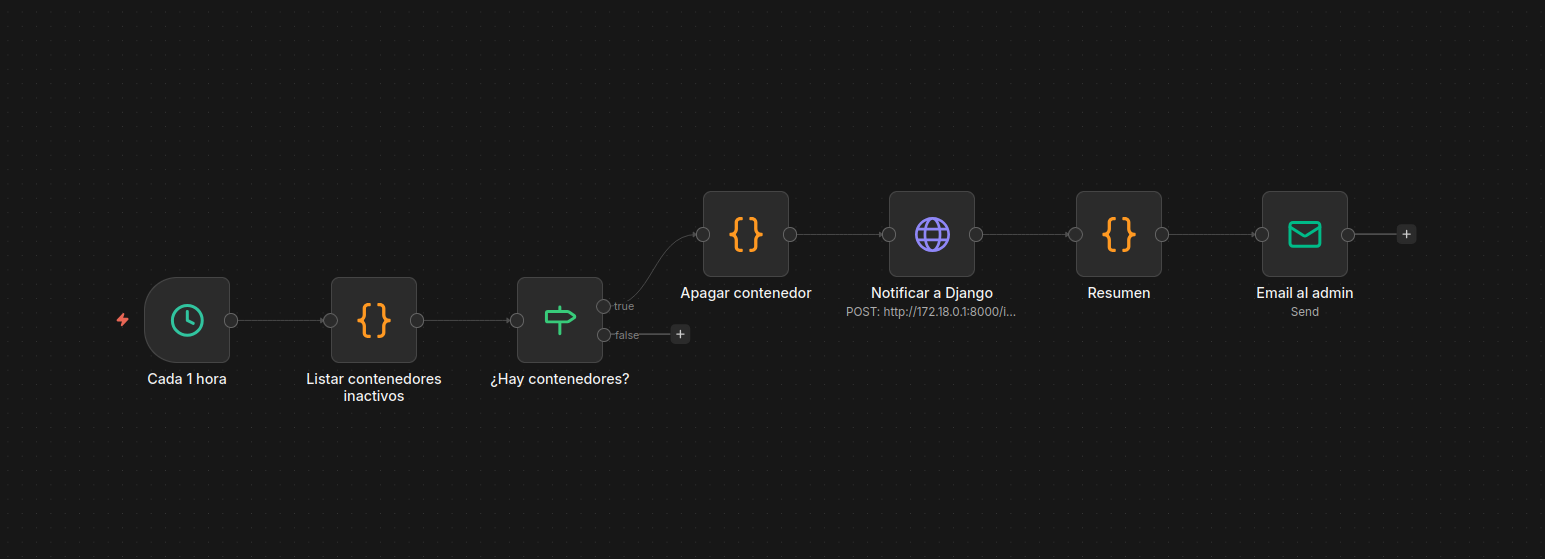
\includegraphics[width=\textwidth]{img/n8n/shutdown.png}
    \caption{Workflow auto shutdown}
    \label{fig:Workflow auto shutdown}
\end{figure}


\subsection{Mejora del workflow de despliegue}
\label{subsec:mejora-workflow-despliegue}

El workflow de despliegue que se había construido en el Sprint 4 carecía de un mecanismo centralizado de gestión de errores. Si cualquiera de los nodos fallaba, la petición de Django quedaba sin respuesta. En este sprint se añadió el nodo \textbf{Responder Error}, que actúa como rama de error compartida para todos los nodos del workflow. Cuando cualquier paso falla, este nodo captura el error y devuelve a Django una respuesta JSON estructurada con el código HTTP 500, un mensaje descriptivo del error y el paso en el que ocurrió. Esto permite que Django actualice el estado del sitio a \texttt{error} y muestre un mensaje útil al usuario, anteriormente se notificaba el error, pero no en detalle.

\begin{figure}[H]
    \centering
    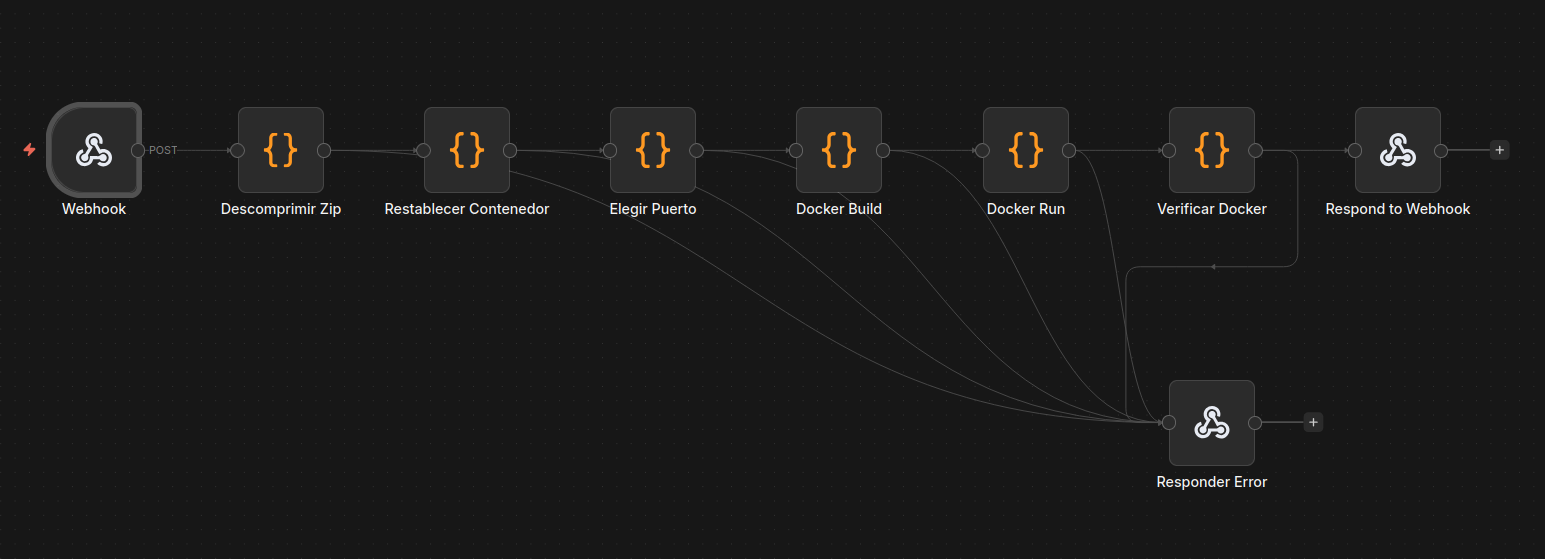
\includegraphics[width=\textwidth]{img/n8n/deploy.png}
    \caption{Workflow deploy}
    \label{fig:Workflow deploy}
\end{figure}


\subsection{Autenticación OAuth con Google y GitHub}
\label{subsec:oauth}

Antes del cierre del proyecto, se integró la autenticación mediante OAuth con Google y GitHub, permitiendo al usuario iniciar sesión o registrarse en WebBuilder con una cuenta ya creada. La autenticación se realizó con la librería \texttt{django-allauth}, que gestiona el flujo OAuth completo y se integra con el sistema de autenticación de Django que ya existía.

\subsubsection{Obtención de credenciales}
Para habilitar el login con Google fue necesario acceder a \textbf{Google Cloud Console}, crear un proyecto OAuth, configurar la pantalla de consentimiento y generar un par de credenciales \texttt{client\_id} y \texttt{client\_secret}. En la configuración del cliente se declaró la URL de redirección, que debe coincidir exactamente con la que allauth espera recibir, es la dirección encargada de devolverte a WebBuilder ya logueado:

\begin{center}
    \texttt{http://\textless{}dominio\textgreater{}/accounts/google/login/callback/}
\end{center}

Para GitHub el proceso es similar, en este caso a través de \textbf{GitHub Developer Settings, OAuth Apps}, donde también se declara la \emph{Authorization callback URL}.

Las credenciales obtenidas se añadieron al fichero \texttt{.env} del servidor como variables de entorno (\texttt{GOOGLE\_CLIENT\_ID}, \texttt{GOOGLE\_CLIENT\_SECRET}, \texttt{GITHUB\_CLIENT\_ID}, \\ \texttt{GITHUB\_CLIENT\_SECRET}) y se leen desde \texttt{settings.py}.


\subsubsection{Arquitectura de la integración}
La integración se compone de tres elementos principales:

\begin{itemize}
    \item \textbf{Adaptador OAuth} (\texttt{WebBuilder/adapters.py}): adaptador personalizado que sobreescribe el comportamiento por defecto de allauth en tres métodos. \texttt{save\_user()} se ejecuta únicamente la primera vez que un usuario accede con OAuth, es decir, en el momento del registro, y dispara el webhook de n8n correspondiente. \texttt{pre\_social\_login()} se ejecuta en cada acceso posterior y dispara el webhook de login con datos del acceso: IP, dispositivo y hora. Por último, \texttt{on\_authentication\_error()} captura cualquier error del flujo OAuth, lo registra en los logs y redirige al usuario a la página de login, evitando que allauth muestre su página de error por defecto sin estilos.

    \item \textbf{Signal \texttt{post\_save}} (\texttt{WebBuilder/signals.py}): garantiza que se cree un \\ \texttt{UserProfile} vacío para cualquier usuario nuevo, independientemente de si se registró mediante el formulario tradicional o mediante OAuth.

    \item \textbf{Templates de allauth} (\texttt{WebBuilder/templates/socialaccount/}): allauth dispone de sus propias páginas HTML para los flujos de autenticación social; cuando no encuentra un template personalizado utiliza los suyos propios, que carecen de estilos. Se crearon templates propios para \texttt{login.html}, \texttt{signup.html} y \\ \texttt{authentication\_error.html} respetando el sistema de estilos del proyecto.
\end{itemize}


\subsubsection{Problemas encontrados durante la puesta en producción}
La integración resultó más compleja de lo esperado por la acumulación de varios problemas independientes que se manifestaban de la misma manera: \emph{Third-Party Login Failure}.

El primer problema fue que la \texttt{SECRET\_KEY} de Django no estaba definida en el \texttt{.env} de producción, por lo que el sistema generaba una clave aleatoria en cada arranque del contenedor. Esto invalidaba las sesiones activas, lo que rompía el flujo OAuth: allauth guarda el parámetro \texttt{state} en la sesión antes de redirigir al proveedor, y si el contenedor se reiniciaba entre la redirección y el callback, la sesión no podía verificarse. La solución fue generar una clave fija y añadirla al \texttt{.env}.

El segundo problema fue el framework \texttt{django.contrib.sites}, que allauth utiliza para construir las URLs de callback, tenía en base de datos el dominio por defecto \texttt{example.com} en lugar del dominio real del servidor. La solución fue editar el registro en el panel de administración de Django (\texttt{/admin/sites/site/}) con el dominio correcto.

El tercer problema fue que las variables \texttt{ALLOWED\_HOSTS} y \texttt{CSRF\_TRUSTED\_ORIGINS} no estaban en el \texttt{.env} de producción pero sí en el local, lo que provocaba que Django rechazara las peticiones del proveedor OAuth. Se añadieron en producción con el dominio del servidor. 

Una vez resueltos todos estos problemas, el flujo OAuth funciona de extremo a extremo: el usuario hace clic en \emph{Login con Google} o \emph{Login con GitHub}, es redirigido al proveedor, selecciona su cuenta y regresa a WebBuilder ya autenticado, con su perfil creado automáticamente y los webhooks de n8n notificados.


\begin{figure}[H]
    \centering
    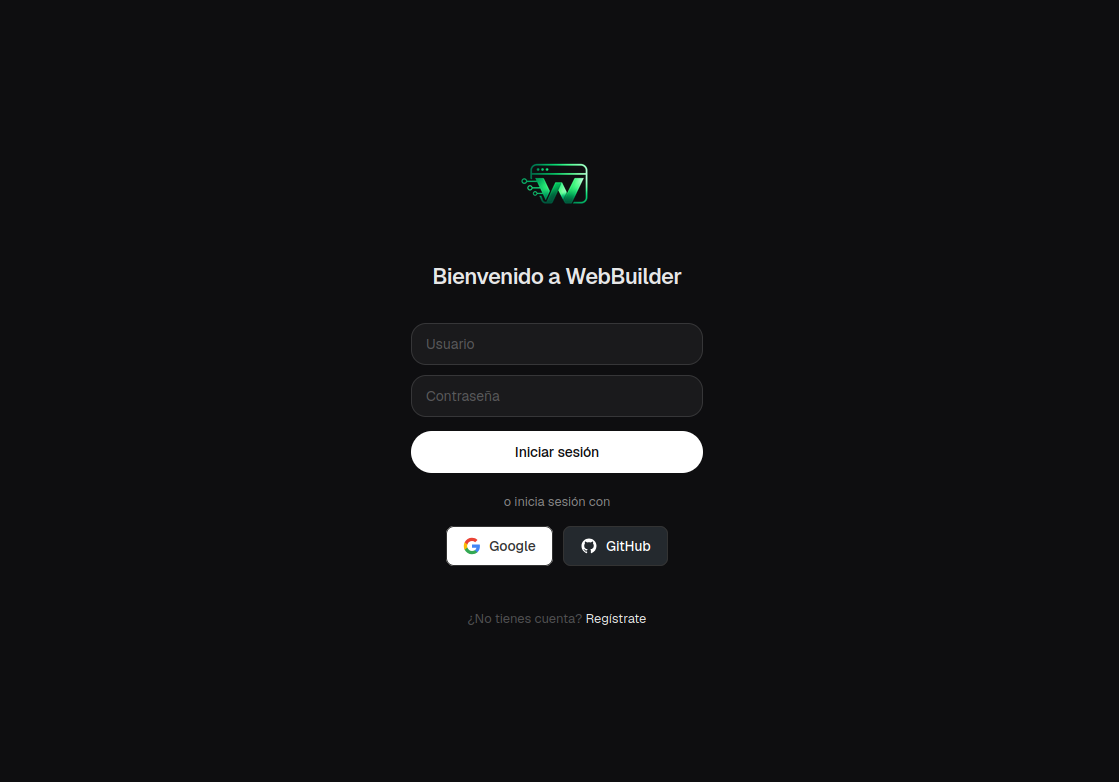
\includegraphics[width=0.9\textwidth]{img/webbuilder/disenoimplementacion/oauth.png}
    \caption{Autenticación Oauth}
    \label{fig:Autenticación Oauth}
\end{figure}
